\documentclass[a4paper,12pt]{article}

\usepackage[dutch]{babel}
\usepackage{fancyhdr}
\usepackage{graphicx}
\usepackage[pdftex,bookmarks=true]{hyperref}
\usepackage[utf8]{inputenc}
\usepackage{fullpage}
\usepackage{parskip}
\usepackage{float}
\usepackage{subcaption}

\title{Samenvatting Ontwerpen III \\ \large HoGent}
\author{Lorenz Verschingel}

\begin{document}
\maketitle
\section{Factory Pattern}
We pakken de code voor de creatie op en verplaatsen deze naar een ander object dat alleen maar het maken van producten als taak zal hebben.
Dit object noemen we \textit{Factory}.

\subsection{Simple Factory}
\begin{figure}[H]
\centering
  	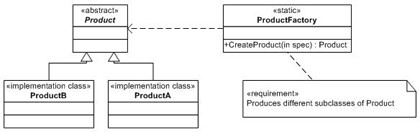
\includegraphics[width=.5\linewidth]{img/Factory/SimpleFactory.jpg}
  	\caption{UML Simple Factory}
  	\label{fig:SimpleFactory}
\end{figure}

Volgens de UML in figuur~\ref{fig:SimpleFactory} kan de ProductFactory producten van het type Product afleveren aan zijn cliënten.

\subsection{Factory Methode}
\begin{figure}[H]
\centering
  	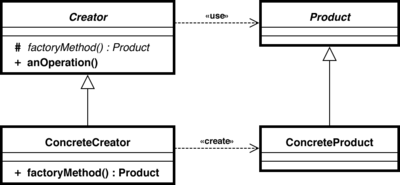
\includegraphics[width=.5\linewidth]{img/Factory/FactoryMethod.png}
  	\caption{UML Factory Methode}
  	\label{fig:FactoryMethod}
\end{figure}

Ten opzichte van figuur~\ref{fig:SimpleFactory} is er niet zoveel veranderd.
In figuur~\ref{fig:FactoryMethod} is de Factory klasse abstract geworden en is de create methode ook abstract.
Deze wordt dan later door een concrete factory geïmplementeerd.

Het Factory Method Pattern definieert een interface voor het creëren van een object, maar laat de subklassen beslissen welke klasse er geïnstantieerd wordt.
De Factory Method draagt de instanties over aan de subklassen.

\subsection{Dependency Inversion-principe}
Wees afhankelijk van abstracties, niet afhankelijk van concrete klassen.

\subsection{Abstract Factory Pattern}
\begin{figure}[H]
\centering
  	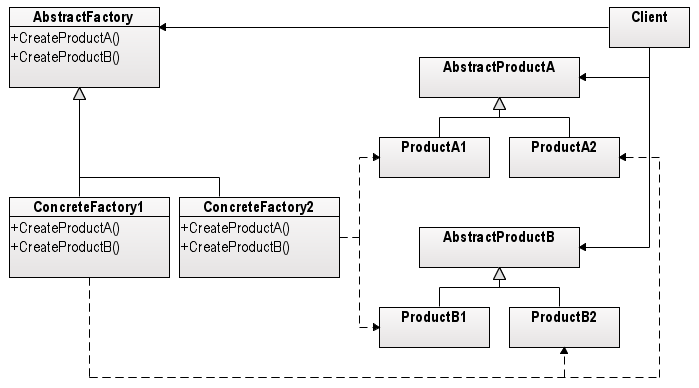
\includegraphics[width=.7\linewidth]{img/Factory/AbstractFactory.png}
  	\caption{UML Abstract Factory}
  	\label{fig:AbstractFactory}
\end{figure}

Het Abstract Factory Pattern levert een interface voor de vervaardiging van reeksen gerelateerde of afhankelijke objecten zonder hun concrete klassen te specificeren.

\section{Iterator Pattern}
\begin{figure}[H]
\centering
  	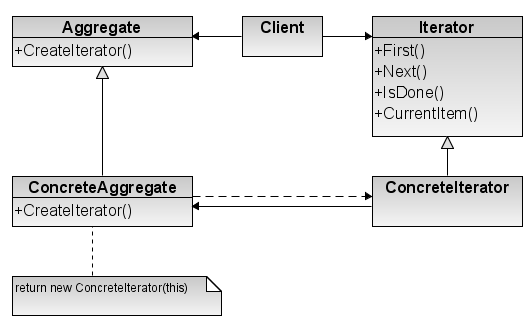
\includegraphics[width=.7\linewidth]{img/Iterator.png}
  	\caption{UML Iterator Pattern}
  	\label{fig:Iterator}
\end{figure}

Het Iterator Pattern voorziet ons van een manier voor sequentiële toegang tot de elementen van een aggregaatobject zonder de onderliggende representatie weer te geven.

Figuur~\ref{fig:Iterator} heeft een redelijk uitgebreide verantwoordelijkheid aan de iterator. In de meeste gevallen volstaat het om een methode hasNext() en Next() in te voeren.

Java voorziet het iterator pattern met de klasse Iterator.
Hiervoor moet men zorgen dat de iterator-klasse de klasse Iterator van Java gebruikt en dat de methode createIterator() het type Iterator$<$teItererenType$>$ terug geeft.
\end{document}